\documentclass[11pt,letterpaper]{article}
\usepackage[lmargin=1in,rmargin=1in,tmargin=1in,bmargin=1in]{geometry}
\usepackage{../style/homework}
\setbool{quotetype}{false} % True: Side; False: Under
\setbool{hideans}{false} % Student: True; Instructor: False

\usepackage{float} % Force Table Placement

% -------------------
% Content
% -------------------
\begin{document}

\homework{9: Due 02/28}{[Penny] God, you know, four years I lived with him. Four years---that's like as long as high school. [Sheldon] It took you four years to get through high school?}{Penny \& Sheldon Cooper, Big Bang Theory}

% Problem 1
\problem{10} Determine whether the relations $F$ and $G$ shown below are functions. Be sure to fully justify your answer. \pspace
	\hfill
	\begin{minipage}[c]{0.48\textwidth}
	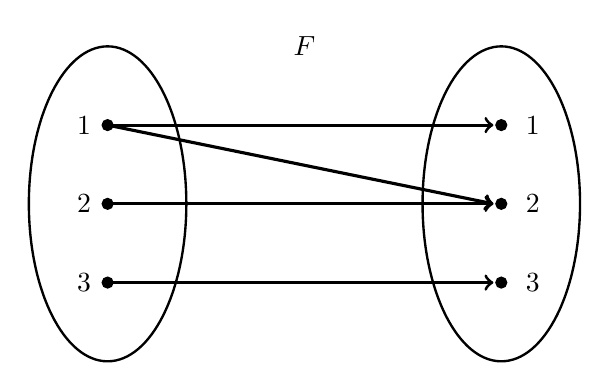
\begin{tikzpicture}
	\node at (2.5,2) {$F$};
	% Ellipses
	\draw[line width=0.03cm] (0,0) circle (1 and 2);
	\draw[line width=0.03cm] (5,0) circle (1 and 2);
	
	% Nodes
	\draw[fill=black] (0,1) circle (0.07);
	\draw[fill=black] (0,0) circle (0.07);
	\draw[fill=black] (0,-1) circle (0.07);
	
	\draw[fill=black] (5,1) circle (0.07);
	\draw[fill=black] (5,0) circle (0.07);
	\draw[fill=black] (5,-1) circle (0.07);
	
	% Arrow
	\draw[line width=0.04cm,->] (0,1) -- (4.9,1);
	\draw[line width=0.04cm,->] (0,1) -- (4.9,0);
	\draw[line width=0.04cm,->] (0,0) -- (4.9,0);
	\draw[line width=0.04cm,->] (0,-1) -- (4.9,-1);
	
	% Labels
	\node at (-0.3,1) {$1$};
	\node at (-0.3,0) {$2$};
	\node at (-0.3,-1) {$3$};
	
	\node at (5.4,1) {$1$};
	\node at (5.4,0) {$2$};
	\node at (5.4,-1) {$3$};
	\end{tikzpicture}
	\end{minipage}%
	\begin{minipage}[c]{0.40\textwidth}
	\begin{table}[H]
	\centering
	\begin{tabular}{cc}
	$x$ & $G$ \\ \hline
	$1$ & $1$ \\
	$2$ & $1$ \\
	$3$ & $1$ \\
	$4$ & $1$ \\
	$5$ & $1$
	\end{tabular}
	\end{table}
	\end{minipage} \pspace \pspace

\sol The relation $F$ is \textit{not} a function because $F(1)$ has more than one possible output, i.e. $F(1)$ is not well defined. However, the relation $G$ is a function because each input has only one possible output---even though all the outputs for $G$ are the same. 



\newpage



% Problem 2
\problem{10} Determine whether the relations $f(x)= 16 - x^2$ and $g(x, y)= \dfrac{x + y}{x - y}$ are functions. Be sure to fully justify your answer. Also, find $f(5)$ and $g(4, 5)$. \pspace

\sol The relation $f(x)$ is a function: for each input $x$, there is only one possible output---namely, the one found by evaluating $f$ at $x$. The relation $g(x, y)$ is a function: for each input $(x, y)$, there is only one possible output---namely, the one found by evaluating $g$ at the given $x, y$. We have\dots
	\[
	\begin{aligned}
	f(5)&= 16 - 5^2= 16 - 25= -9 \\[0.3cm]
	g(4, 5)&= \dfrac{4 + 5}{4 - 5}= \dfrac{9}{-1}= -9
	\end{aligned}
	\]



\newpage



% Problem 3
\problem{10} Suppose $f(x)$ and $g(x)$ are the functions given below. 
	\[
	\begin{aligned}
	f(x)&= 1 - 4x \\[0.3cm]
	g(x)&= x^2 + 1
	\end{aligned}
	\]

Compute the following: \pspace
        \begin{enumerate}[(a)]
        \item $6f(1) - g(2)= 6 \big(1 - 4(1) \big) - (2^2 + 1)= 6(-3) - (4 + 1)= -18 - 5= -23$ \vfill
        \item $(f + g)(1)= f(1) + g(1)= \big(1 - 4(1) \big) + (1^2 + 1)= -3 + 2= -1$ \vfill
        \item $(f - g)(0)= f(0) - g(0)= \big(1 - 4(0) \big) - (0^2 + 1)= 1 - 1= 0$ \vfill
        \item $(fg)(2)= f(2) \cdot g(2)= \big(1 - 4(2) \big) \cdot (2^2 + 1)= -7 \cdot 5= -35$ \vfill
        \item $(f \circ g)(-1)= f \big( g(-1) \big)= f \big( (-1)^2 + 1 \big)= f(1 + 1)= f(2)= 1 - 4(2)= 1 - 8= -7$ \vfill
        \item $(g \circ f)(-1)= g \big( f(-1) \big)= g \big( 1 - 4(-1) \big)= g(1 + 4)= g(5)= 5^2 + 1= 25 + 1= 26$ \vfill
        \end{enumerate} 


\end{document}